% System_Overview.tex
% replaces Problem Definition and Customer Base
\section{System Overview}

%% System Requirements from beginning/PPFS
%\subsection{System Requirements -- TBD}   % not including this here since we have a full section just for requirements
%To be included...

%% System block diagram
\subsection{System Block Diagram}
\begin{figure}[htbp]
  \centering
  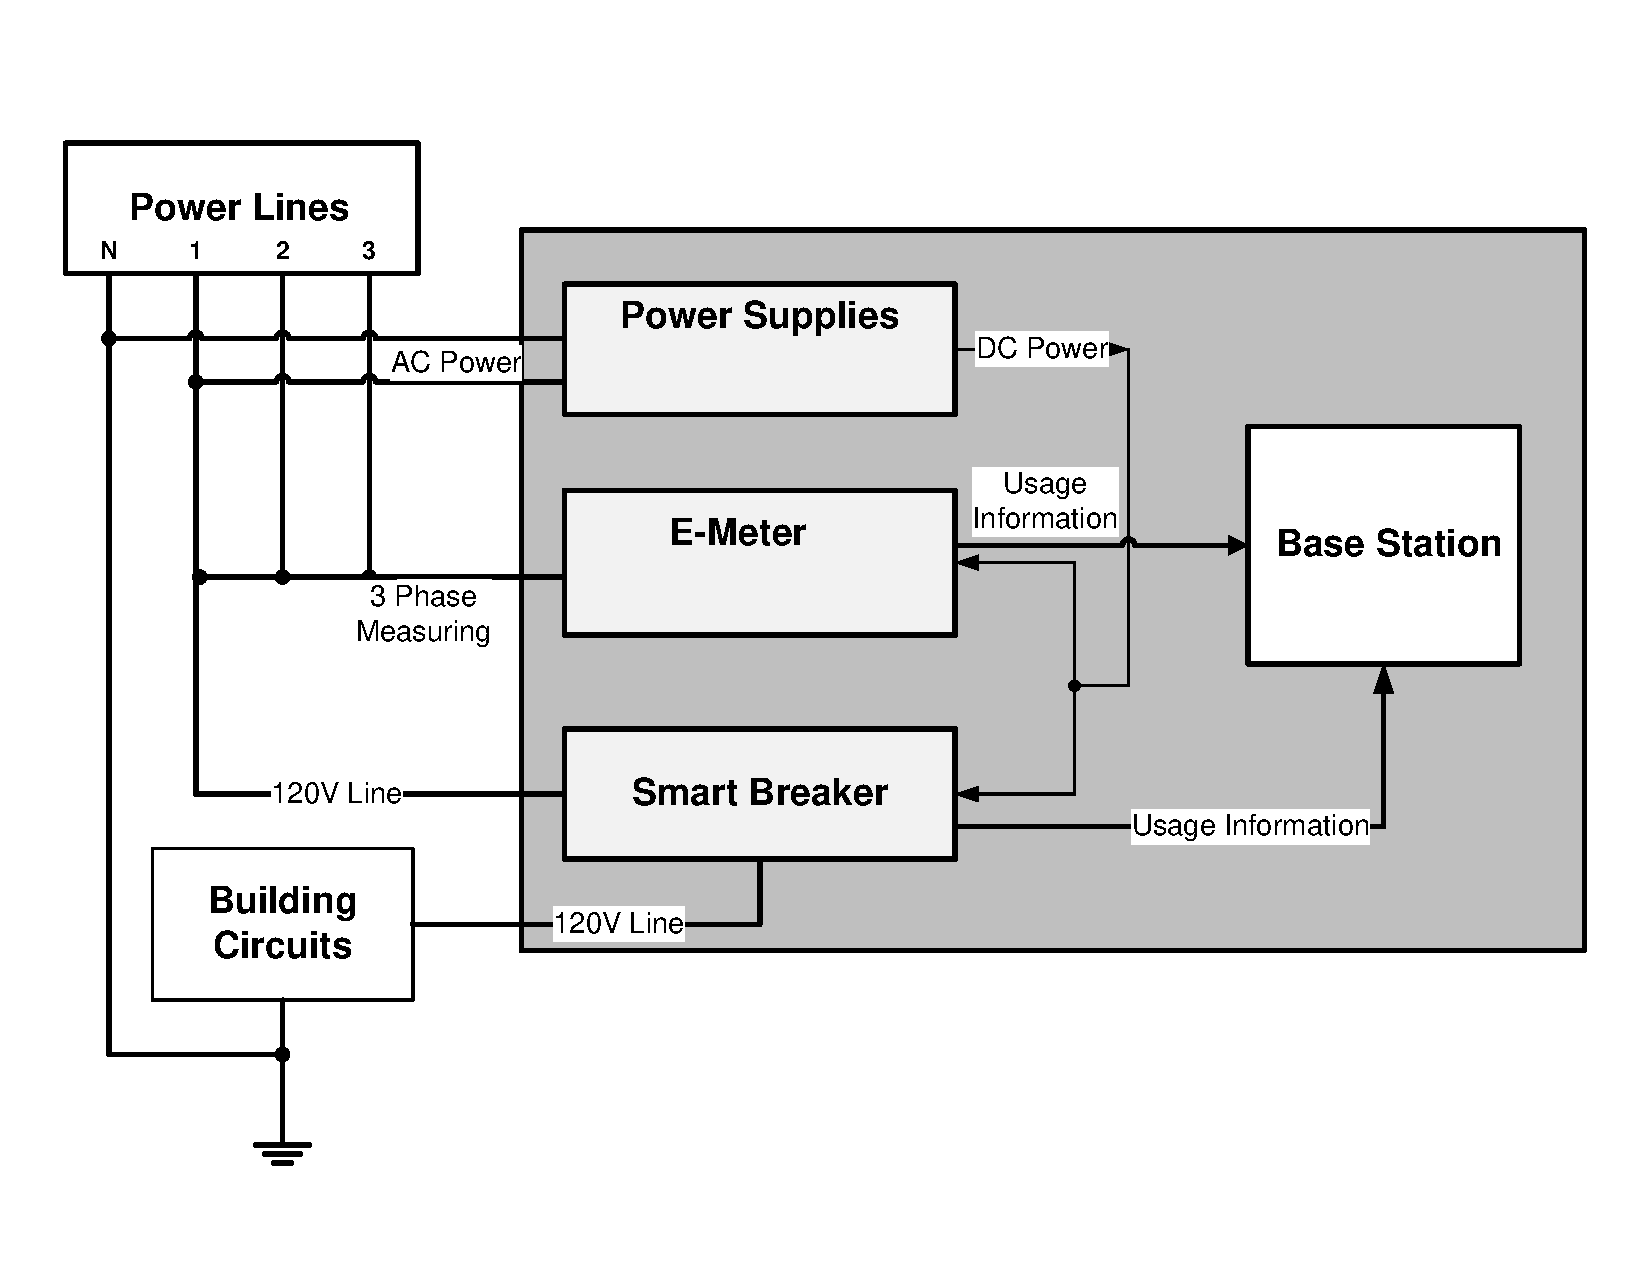
\includegraphics[width=\textwidth]{includes/PICA_System_Diagram_B}
  \caption{System block diagram}
  \label{fig:system_block_diagram}
\end{figure}

%% System Explantion
\subsection{System Explanation}

The full PICA system consists of the e meter, base station, smart breakers and power supply. The system was designed to minimize dependencies between subsystems, allowing the user to choose which information they want without paying for more than that. The fact that the power company and homeowner both have an interest in the PICA system drove much of this decision. As two customers with different requirements, neither party would want to pay to provide the other with information that isn't useful to the first. The team wanted both parties to have information if they wanted it without forcing unwanted costs on one party or the other. The team later decided that designing for the power company was not feasible. However, keeping the subsystems as independent as possible allows for continued development with the power company's interests in mind should another team work on the project later.

The e meter measures power for the entire building and provides information to the power company. The built in display allows the e meter to operate and provide information completely independently of the base station, although the Xbee connection allows viewing of the information through the base station if desired. The e meter is dependent on the power supply.

The base station is targeted at the homeowner, providing a simple and easy way of viewing information collected by other parts of the system. While the e meter and breakers are not required for the base station to run, it would have no information to provide, and would therefore be useless. Because the base station provides no controls for the other subsystems, it is not required for the other subsystems to operate properly. The base station is not dependent on the power supply. After a lot of work on the base station, the team decided to focus on the e meter and smart breakers and use a standard computer in place of the dedicated base station for prototyping and testing.

The smart breakers provide circuit breaker level information to the homeowner, in addition to providing the same functionality as standard air-gap breakers. The smart breaker's only means of displaying the information is through the base station, so to provide useful data the smart breakers are dependent on the base station. However, the smart breakers still function as breakers without the base station. This is important so that a problem with the base station doesn't shut off power to all of the smart breaker circuits. The smart breakers are also dependent on the power supply.

The power supply provides power to the E-Meter and Smart Breakers and is placed so that it is still able to power everything when all of the breakers are shut off. This is important because the smart breakers' default state is off and won't turn on until they have power, so if the smart breaker came before the power supply, the system would never turn on. 

%% Testing
\subsection{Testing}
Once each subsystem passes its respective verification plan, the three PICA systems can begin integration testing. The system level integration testing verifies that all systems are capable of talking to one another under normal operating conditions.
\subsubsection{Simple Talk Test}
This test verifies that all systems are capable of talking to one another. Begin by placing both the smart meter and the breaker in a situation where they are guarenteed to talk, such as monitoring an active load. Attach a computer to each device, verifying that in fact they are correctly sending data. Once each system has been verified to be operational, attach Xbee radio cards to the prototype boards and a computer console to the base station. Verify that data transmitted from each device is received by the base station computer. The team expects that data received at the base station will be identical to data seen leaving each device.

\subsubsection{Simple Command Test}
This test verifies that the base station is capable of sending various commands to the individual subsystems. After all systems have been powered on and placed in an operation state, send the `q' command out across the Xbee network. This should result in both systems halting in an expected fashion. The E-Meter should cease taking measurements and blank the screen while the Smart Breaker changes to the Off state. At this time, both should stop talking.

Continue this test by trying this command an additional time, but specifying which subsystem should respond to the command. Test the E-Meter and Smart Breaker individually, each time sending the `q' command. The response should be the same, but only the device specified should halt.

\subsubsection{Complex Command Test}
Repeat the previous test, using more complex commands asking for specific information. Commands can be seen in the table \ref{tab:pica_system_commands}.
\begin{table}[htbp]
  \centering
  \begin{tabular}{|c|p{2in}|}\hline
    Command & Behavior \\\hline\hline
    q     & Kills the system \\\hline
    b\#    & Specifies a breaker to command\\\hline
    m     & Specifies the command is for the E-Meter\\\hline
    v [\#] & Specifies that voltage should be reported. An optional number is allowed for sending to the meter to select which phase.\\\hline
    i [\#] & Identical to v except returns current.\\\hline
    p [\#] & Identical to v except returns power.\\\hline
    wh    & Returns the accumulated watt-hours.\\\hline
    s     & Used in conjunction with a breaker to return its status.\\\hline
  \end{tabular}
  \caption{PICA System commands.}
  \label{tab:pica_system_commands}
\end{table}
As a result of sending any one of these commands, either all or the specified system should return the data requested.

\subsubsection{Web Interface Test}
Verify that the system is properly reporting data to the web interface and rerun all tests through the web interface command line. Results should match those seen in previous tests.
%Basic Xbee tests proved it is a viable option for communication between subsystems.

%Some testing was completed, using the standard computer and e meter. [Pictures of perl 'base station' should go in this section]

%Testing between the smart breakers and base station need to be completed once the smart breakers are functional.
%which isn't really true since we could have generated numbers with the Arduino and just used that...

%% Future Work
%\subsection{Future Work -- TBD}